\section{Hybrid Policies}

Le policy ibride servono per garantire sia la confidenzialità che l'integrità.
Le principali sono: modello a Muraglia Cinese (\textbf{Chinese Wall}) basato sul
concetto di conflitto di interesse; \textbf{ORCON} che combina le regole di
controllo sugli accessi di tipo mandatory con quelle di tipo discretionary;
\textbf{RBAC} dove l'accesso avviene tramite regole di controllo basate sui
ruoli di appartenenza (usato in ambienti commerciali come SAP).

\subsection{Chinese Wall}

La politica della “\textit{muraglia cinese}” è stata introdotta da Brewer e Nash
nel 1989 per evitare che informazioni sensibili, concernenti una certa compagnia,
vengano passate a compagnie rivali per mezzo di consulenti finanziari.
Si stabiliscono dinamicamente i diritti di accesso degli utenti in base
alle risorse a cui l'utente stesso ha già avuto accesso.
Tale modello organizza le entità in classi basate su \textit{Conflitti di Interesse}.
Il controllo sull'utente
viene effettuato prima dell'accesso ad ogni classe e al momento della scrittura,
in questo ultimo
caso il controllo viene fatto su tutte le classi per avere la certezza che
l'informazione non violi le
regole sui conflitti di interesse. Per ogni classe di conflitto di interesse
saranno definite delle
informazioni visibili a tutti chiamate “\textbf{Sanitized Data}”
(informazioni prive di dati sensibili).
Occorre definire tre elementi:

\begin{itemize}
    \item \textit{Oggetti} (\textbf{O}): sono gli elementi di informazione
          relativi ad un'azienda;
    \item \textit{Company Dataset} (\textbf{CD}): contiene l'insieme degli
          oggetti relativi ad una singola azienda
          (l'operazione di inserimento di un oggetto è chiamata \(CD(o)\));
    \item \textit{Conflict of Interest Class} (\textbf{CoI}): contiene
          l'insieme delle aziende in concorrenza tra di
          loro (l'operazione di inserimento di un'azienda è detta \(CoI(o)\));
          ogni oggetto appartiene
          esattamente a una classe CoI.
\end{itemize}

Prendiamo in esame la seguente immagine:

\begin{figure}[H]
    \centering
    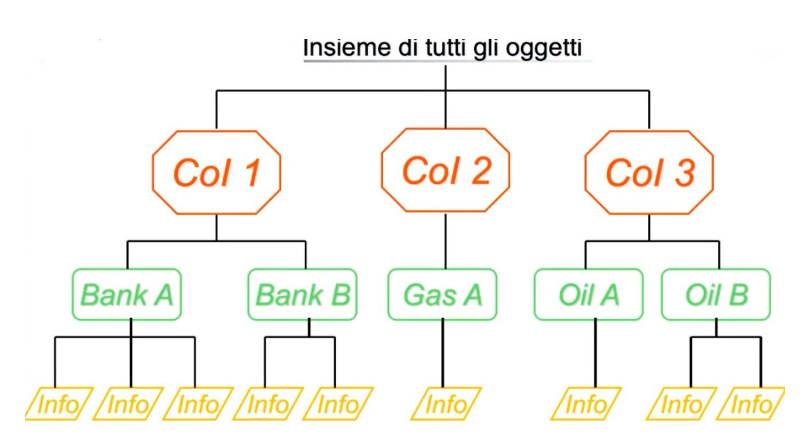
\includegraphics[width=10cm, keepaspectratio]{capitoli/policy/imgs/chinese1.png}
\end{figure}

Gli oggetti \textit{O} solo le “Info”. I \textit{CD} sono \verb|Bank A|
e \verb|Bank B|, \verb|Gas A|, \verb|Oil A| e \verb|Oil B|.
Le banche \verb|A| e \verb|B| sono
in conflitto tra loro e per questo nella
medesima \textit{CoI} indicata con 1. Gli altri CD
appartengono alle \textit{CoI} 2 e 3.
Il protocollo vuole evitare che se un
consulente accede ai dati della banca \verb|A|, non
può accedere a quelli della banca \verb|B| perché
esse sono chiaramente in conflitto.
Quindi, se un consulente legge un oggetto appartenente ad un \textit{CD} in una
data \textit{CoI}, non può più
leggere oggetti di altri \textit{CD} in quella \textit{CoI}.
È possibile che le informazioni apprese prima possano consentirgli di prendere
decisioni “migliori” dopo (ovviamente in modo sleale).
Indichiamo con \(PR(S)\) l'insieme degli oggetti che \textit{S} ha già letto.
Una semplice condizione di sicurezza in fase di lettura, prevede che un soggetto
\textit{S} può leggere un
oggetto \textit{O} se e solo se:

\begin{itemize}
    \item Esiste un oggetto \(o'\) a cui \textit{S} ha avuto accesso e
          \(CD(o') = CD(o)\) oppure
    \item Per ogni \(o' \in O, \ o' \in PR(S) \Rightarrow CoI(o') \neq CoI(o)\).
\end{itemize}

\(o\) (minuscolo) è un oggetto sanitized e perciò non genererà conflitti di
interesse.
In questa politica non vengono presi in considerazione i dati sanitized ed
inizialmente \(PR(S) = \emptyset \).
In altri termini, un soggetto può leggere un oggetto se l'oggetto è in un dataset
di cui il soggetto ha
già letto qualcosa oppure l'oggetto appartiene a una \textit{CoI} di cui il
soggetto non ha letto ancora niente. Nel nostro esempio, se il consulente legge
dalla banca \verb|A| non potrà leggere dalla \verb|B|. Non
appena viene compiuta un'azione di lettura viene negato l'accesso ad altri dati
che potrebbero generare conflitti di interessi.
La politica \textbf{Chinese Wall} è una combinazione di \textit{libera scelta} e
\textit{MAC}. Inizialmente un soggetto è
libero di accedere a ciò che vuole ma, una volta effettuata la scelta, per
quell'utente viene creata una \textit{Muraglia Cinese} attorno al dataset a cui
l'oggetto appartiene.
Si noti che la Chinese Wall può essere combinata con le politiche DAC.

\paragraph{Esempio.}
Anthony e Susan lavorano per la stessa azienda di consulenza.
Anthony può leggere i \textit{CD} di \verb|Bank A| e di \verb|Gas A| e Susan
può leggere i \textit{CD} di \verb|Bank B| e di \verb|Gas A|. Se Anthony potesse
scrivere sul \textit{CD} di \verb|Gas A|, Susan potrebbe leggerlo. Perciò,
indirettamente, potrebbe acquisire informazioni su
\verb|Bank B|, un chiaro conflitto di interesse. La regola così descritta per la
lettura non è in grado di prevenire “fughe di notizie”.\\

Quindi, in fase di scrittura, il modello deve stabilire che un soggetto \textit{S}
può scrivere un oggetto \(o\) se e solo se:

\begin{enumerate}
    \item La condizione di sicurezza in lettura permette a \textit{S} di
          leggere \(o\),
    \item Per ogni oggetto non \textit{sanitized} (quindi sensibile) \(o'\),
          se \textit{S} può leggere \(o'\), allora \(CD(o') = CD(o)\).
\end{enumerate}

In pratica \textit{S} può scrivere un oggetto se tutti gli oggetti sensibili
che può leggere appartengono allo stesso dataset. Un utente che ha letto più
\textit{CD} non potrà scrivere nessun oggetto; inoltre, una volta
che ha scritto in un \textit{CD}, potrà scrivere soltanto lì.
Così il flusso di informazioni è destinato a restare all'interno dell'azienda.
In altri termini, un
soggetto può scrivere un oggetto se lo può anche leggere e non può leggere dati
di altre compagnie.

\subsubsection{Chinese Wall vs Bell-LaPadula}

Chinese Wall non assegna etichette di sicurezza
ma si basa sugli accessi passati. Bell-LaPadula può
simulare Chinese Wall istante per istante, in questo
caso: ogni coppia di \verb|(CoI, CD)| costituirà una
categoria, ci saranno due livelli di sicurezza (\textit{S}
(sanitized), \textit{U} (non sanitized), in cui \textit{S} domina \textit{U}),
ad ogni soggetto deve essere associata al massimo
una sola categoria per ogni classe \textit{CoI}. Però,
Bell-LaPadula non sarà in grado di gestire gli
accessi passati e di adattare i vincoli relativi ai
permessi di accesso con il variare del tempo (in
Chinese Wall infatti, inizialmente si ha accesso a
tutti gli oggetti, poi no).

\subsubsection{Chinese Wall vs Clark-Wilson}

Se non è prevista una distinzione tra i soggetti
ed i processi, allora si rispetterebbe il modello
di Clark-Wilson ma si violerebbe il modello
Chinese Wall (una singola persona può
accedere a più processi). Se però è prevista
una separazione tra soggetto e processo allora
si dovrebbero rispettare entrambi i modelli in
termini di sicurezza di integrità.

\subsection{ORCON \normalfont\emoji{ogre}}

Il modello ORCON stabilisce che i diritti di accesso vengono definiti
dall'utente che ha creato l'oggetto. Il diritto di lettura di un dato non è
concesso al possessore del dato ma a colui che l'ha
originato.

\begin{enumerate}
    \item Il soggetto \(s \in S\) marca l'oggetto \(o \in O\) come ORCON per
          conto dell'organizzazione \(X\).
    \item \(X\) permette che \(o\) sia diffuso ai soggetti che lavorano per
          conto dell'organizzazione \(Y\) con le seguenti restrizioni:
          \begin{itemize}
              \item \(o\) non può essere rilasciato a soggetti che lavorano per
                    conto di altre organizzazioni senza il permesso di \(X\);
              \item Ogni copia di \(o\) deve avere le stesse restrizioni.
          \end{itemize}
\end{enumerate}

Per realizzare questa politica non sono idonei nè \textit{MAC} nè \textit{DAC}.
DAC non può essere utilizzato poiché il possessore potrebbe concedere qualsiasi
diritto violando la seconda proprietà.
MAC è inadeguato poiché:

\begin{itemize}
    \item può causare un'esplosione del numero di categorie;
    \item la gestione degli accessi avviene in maniera centralizzata,
          mentre in ORCON è richiesta
          una gestione locale.
\end{itemize}

La soluzione prevede la combinazione di MAC e DAC generando la seguente tecnica
di gestione degli accessi: il possessore dell'oggetto non può cambiare i
controlli di accesso. Quando l'oggetto
viene copiato, vengono copiate anche le restrizioni di accesso dalla sorgente
(cioè è MAC, il possessore non può controllarlo); il creatore del documento può
alterare le restrizioni di accesso in base al soggetto e all'oggetto
(cioè è DAC, il creatore può controllarlo).

\subsection{RBAC}

Il modello \textbf{RBAC} (\textit{Role Based Access Control}) nasce poiché un
problema importante nell'organizzazione di grandi sistemi è la complessità
dell'amministrazione della sicurezza.
Quando il numero dei soggetti e degli oggetti è alto, il numero di autorizzazioni
può diventare molto grande.
Inoltre, se l'utenza è dinamica, il numero di concessioni e di revoche di permessi
diventa davvero elevato. Gli utenti finali spesso non “possiedono” le informazioni
a cui hanno accesso. Le aziende o gli enti sono i reali possessori degli oggetti.
Il controllo di accesso è quindi basato sulle mansioni delle persone e non sul
semplice possesso.
RBAC è stato quindi proposto come alternativa al DAC e al MAC per semplificare
la gestione degli accessi e per supportare direttamente il controllo basato sui
ruoli.
I diritti di accesso dipendono dal ruolo del soggetto ma non dalla sua identità.
I ruoli rappresentano le mansioni all'interno di un'organizzazione;
le autorizzazioni sono concesse ai ruoli anziché ai
singoli utenti. Gli utenti sono perciò autorizzati semplicemente ad assumere ruoli
appropriati, acquisendo le autorizzazioni assegnate a quei ruoli.
Poiché i ruoli rappresentano le funzioni dell'organizzazione, un modello RBAC può
direttamente supportare le politiche di sicurezza proprie dell'organizzazione.
La concessione e la revoca delle
autorizzazioni alle categorie di utenti è estremamente semplificata.
I modelli RBAC sono anche detti “\textbf{policy-neutral}”.

\subsubsection{Modello RBAC-NIST}

Il modello RBAC NIST è una definizione standard di controllo di accesso basato
sui ruoli. Nel 2000, il NIST ha richiesto uno standard unificato per RBAC,
integrando il modello RBAC pubblicato nel 1992.
Il modello dispone di \textbf{tre} livelli con capacità funzionali crescenti:
\textbf{Core RBAC} (o Flat RBAC), \textbf{RBAC Gerarchico}, \textbf{RBAC Vincolato}.
Formalmente, RBAC definisce:

\begin{itemize}
    \item \textbf{Utente}: un essere umano, una macchina, un processo, o un
          agente intelligente autonomo, ecc.;
    \item \textbf{Ruolo}: una funzione nel contesto di un'organizzazione con
          una semantica associata
          secondo l'autorità e la responsabilità del ruolo;
    \item \textbf{Permesso}: modo di accesso che può essere esercitato sugli
          oggetti nel sistema.
    \item Sia gli oggetti e i modi di accesso sono dipendenti dal dominio;
    \item \textbf{Sessione}: è una particolare istanza di una connessione di
          un utente al sistema e definisce
          un sottoinsieme di ruoli attivati.
    \item Ad ogni istante, possono essere attive più sessioni differenti per
          ciascun utente.
    \item Quando un utente entra nel sistema, stabilisce una sessione e durante
          tale sessione può
          attivare un sottoinsieme dei ruoli che è autorizzato ad assumere;
    \item L'utente ottiene i permessi associati al ruolo che ha attivato nella
          sessione
\end{itemize}

\paragraph{RBAC Float.}

In questo primo modello vengono definiti solo gli elementi essenziali senza i
quali non è possibile implementare un controllo d'accesso.

\begin{itemize}
    \item il \textbf{ruolo} è un insieme di funzioni; \verb|trans(r)|
          indica le transazioni autorizzate per il ruolo \verb|r|;
    \item I ruoli attualmente attivi per il soggetto \verb|s| sono dati da
          \verb|actr(s)|;
    \item il set di ruoli autorizzati per il soggetto \verb|s| si calcolano
          con \verb|authr(s)|;
    \item le azioni che il soggetto \verb|s| può fare al tempo \verb|t| si
          ricavano da \verb|canexec(s, t)| il cui risultato
          dipende dal ruolo di \verb|s|.
\end{itemize}

Sia \verb|S| l'insieme dei soggetti e \verb|T| quello delle transazioni:
le transazioni che il soggetto può fare
dipendono dal ruolo di \verb|s|; i ruoli che \verb|s| ha attivi sono un
sottoinsieme dei ruoli autorizzati per \verb|s|.
Se \verb|t| è una transazione che il soggetto \verb|s| può eseguire, allora essa
è anche una di quelle transazioni permesse a tutti i soggetti del ruolo
ricoperto da \verb|s|.

\paragraph{RBAC Gerarchico.}
La gerarchia tra i ruoli è un modo naturale per strutturarli, riflettendo le
linee di autorità e responsabilità di un'organizzazione. Ad un ruolo
gerarchicamente più importante, saranno assegnate le stesse azioni di un ruolo
meno importante più alcune specifiche, ovvero:

\[
    (\forall s \in S)[ \ r' \in authr(s) \wedge r' > r \rightarrow r \in authr(S) \ ]
\]\footnote{È inutile ed incomprensibile, ma era carina da vedere.}

In tale modello è applicabile il principio di ereditarietà:

\begin{itemize}
    \item \textit{Ereditarietà di utente} (\textbf{UI}): Tutti gli utenti
          autorizzati ad un ruolo \verb|r| sono anche autorizzati ad
          un ruolo \verb|r'|, ove \(r > r'\)
    \item \textit{Eredità di permessi} (\textbf{PI}): Un ruolo \verb|r| è
          autorizzato a tutti i permessi per i quali ogni ruolo \verb|r'|,
          tale che \(r > r'\), è autorizzato
    \item \textit{Eredità di attivazione} (\textbf{AI}): Attivando un
          ruolo \verb|r| automaticamente si attivano tutti i ruoli \verb|r'|,
          tali che \(r > r'\).
\end{itemize}

\paragraph{RBAC Vincolato.}
È un modello RBAC con la capacità di supportare le politiche di
\textit{Separazione dei compiti}
(\textbf{Separation of Duty}). Evita conflitti di interesse e collisioni tra
mansioni.
Sia \verb|r| un ruolo e \verb|s| un soggetto tale che \verb|r|
appartiene a \verb|auth(s)|, allora il predicato
\verb|meauth(r)| (usato per assegnare autorizzazioni in mutua esclusione) è
l'insieme dei ruoli che \verb|s| non può assumere a
causa dei requisiti di separazione dei
compiti.

\[
    (\forall r_1, r_2 \in R) [ \ r_2 \in meauth(r_1) \rightarrow
            [ \ (\forall s \in S) [ \ r_1 \in authr(s) \rightarrow r_2 \notin authr(s) \ ] \ ] \ ]
\] \footnote{Anche questa è inutile ed incomprensibile, ma carina da vedere.}

In pratica, la \textit{Separation of Duty} stabilisce che
se un ruolo \(r_2\) è in conflitto con un ruolo \(r_1\),
allora ogni soggetto \verb|s| autorizzato al ruolo \(r_1\)
non può essere autorizzato al ruolo \(r_2\).
Esistono due tipi di categorie di separazione dei compiti (Separation of Duty):

\begin{itemize}
    \item \textbf{Statici}: restringono l'insieme dei ruoli, ed in particolare
          la possibilità di entrare nella
          relazione RA. Per evitare che una persona sia autorizzata ad assumere
          troppi ruoli, nessun
          utente può assumere più di un certo numero di ruoli in un determinato
          insieme di ruoli;
    \item \textbf{Dinamici}: limitano il numero di ruoli che un utente può
          attivare in una singola sessione.
          Ad esempio si può stabilire un massimo numero di ruoli in una sessione,
          oppure si può stabilire che se assunto un ruolo in una sessione non
          si possono assumere altri ruoli nella stessa
          sessione. Ovviamente per garantire questa tecnica di assegnamento
          dei compiti, è
          importante mantenere una storia dei ruoli attivati da ciascun
          utente nell'arco della sessione.
\end{itemize}

In conclusione, le politiche ibride riguardano sia la riservatezza che l'integrità.
Diverse combinazioni di questi modelli ORCON non sono né MAC né DAC.
In realtà, un modello RBAC combinato controlla l'accesso in base alle funzionalità.